%%%%%%%%%%%%%%%%%%%%%%%%%%%%%%%%%%%%
%% Template file SP 2024
%% Include in directory homework.sty and headerfooter.tex
%%%%%%%%%%%%%%%%%%%%%%%%%%%%%%%%%%%%

\documentclass[12pt]{article}
\usepackage{homework}

\graphicspath{{images/}}
\geometry{letterpaper, portrait, includeheadfoot=true, hmargin=1in, vmargin=1in}

\setcounter{section}{-1}
%% Solution hiding %%
\usepackage[utf8]{inputenc}
\usepackage{lipsum}


\begin{document}
\singlespacing

\renewcommand{\familydefault}{\rmdefault}
\pagestyle{fancy}
\fancyhf{}
\setlength{\headheight}{30pt}
\renewcommand{\headrulewidth}{0.4pt}
\renewcommand{\footrulewidth}{0.4pt}
\lhead{\large Homework 2 \\ Due Feb. 20, 2024 }
\rhead{\large CS 446 \\ Spring 2024}
\rfoot{\textbf{Page \thepage}}
\lfoot{}

\section{Instructions}

Homework is due Tuesday, March 18, 2024 at 23:59pm Central Time.
Please refer to \url{https://courses.grainger.illinois.edu/cs446/sp2024/homework/hw/index.html} for course policy on homeworks and submission instructions.

\section{Neural networks for simple functions}
\subsection{}
\begin{eqnarray}
    \omega_{0} = (1, -1)^T  \omega_{1} = (1, -1)^T \nonumber
\end{eqnarray}

\subsection{}
\begin{eqnarray}
    \omega_{0} = (1, -1)^T  \omega_{1} = (1, -1)^T b = (1, -1)^T \nonumber
\end{eqnarray}

\subsection{}
\begin{eqnarray}
    \omega_{0} = 0  \omega_{1} = 2b  \nonumber
\end{eqnarray}

\subsection{}
\begin{eqnarray}
    \omega_{0} = (3, -6, 3)^T b = (6, 0, -6)^T \omega_{1} = (1, -1, 1)^T \nonumber
\end{eqnarray}

\subsection{}
No. ReLu makes negative part of the innner linear function to 0, and positive parts to remain the same. So, after applying the outter linear function, the output will also be a combination of a linear function and a 0 part.

\subsection{}
No. Suppose $x_{0}$ satisfies $|w_1^T\sigma(w_0^T x_0 + b) - x_0^2| < \epsilon$, as $x_{0}$ goes to infinity, the $x_0^2$ increases at a second order rate, while the first term increases at a maximum first order rate. So, the difference will go to infinity.

\subsection{}
Yes. For any small $\epsilon$, we can find a large enough amount of line segments to approximate the quadratic function. 

The construction routine is as follows.

Suppose the line segments are $l_0, l_1, \dots, l_n$. The objective $w_1^T \sigma(w_0 x + b_0)$ can be viewed as a linear combination of $\sigma(w_0^0 x + b_0^0), \sigma(w_0^1 x + b_0^1), \dots, \sigma(w_0^m x + b_0^m)$.
We can choose $w_0^0 x + b$ to be the line containing the segment $l_0$. Then, for every $i \ge 1$ choose $w_0^i$ equal to the differnce between the slope rate of segment $i$ and segment $i+1$, $b_0^i$ equal to the corresponding intersection when the line $w_0^i x + b_0^i = 0$. $w_1 = (1, 1, \dots, 1)$
\newpage

\section{Backpropagation through time (BPTT)}
\subsection{}
\begin{figure}[h]
    \centering
    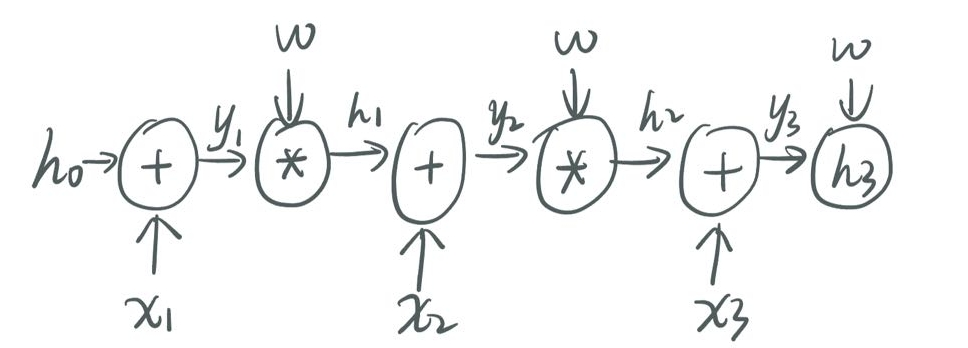
\includegraphics[width=0.8\textwidth]{imgs/2-1.jpg}
    \caption{Illustration of 2.1}
    \label{fig:2-1}
\end{figure}

\subsection{}
\begin{align}
    &h_0 = 0 \quad y_1 = h_0 + x_1 \nonumber  \\
    &h_1 = w^T (h_0 + x_1) \quad  y_2 = w^T(h_0 + x_1) + x_2 \nonumber  \\
    &h_2 = w^T(w^T(h_0 + x_1) + x_2) \quad  y_3 = w^T(w^T(h_0 + x_1) + x_2) + x_3 \nonumber  \\
    &h_3 = w^T(w^T(w^T(h_0 + x_1) + x_2) + x_3) \quad \nonumber
\end{align}

\subsection{}
\begin{eqnarray}
    \frac{\partial h_3}{\omega} &=& y_3 + \omega \frac{\partial y_3}{\omega} \nonumber \\
    &=& y_3 + \omega \frac{\partial h_2}{\omega} \nonumber \\
    &=& y_3 + \omega (y_2 + \omega \frac{\partial y_2}{\omega}) \nonumber \\
    &=& y_3 + \omega y_2 + \omega^2 \frac{\partial h_1}{\omega} \nonumber \\
    &=& y_3 + \omega y_2 + \omega^2 (y_1 + \omega \frac{\partial y_1}{\omega}) \nonumber \\
    &=& y_3 + \omega y_2 + \omega^2 y_1 \nonumber
\end{eqnarray}

\subsection{}
\begin{eqnarray}
    \frac{\partial f}{\partial h_1} &=& \frac{\partial f}{\partial h_T} \frac{\partial f}{\partial h_{T-1}} \dots \frac{\partial h_2}{\partial h_1} \nonumber \\
    &=& 1 \cdot \omega \sigma'(x_t + h_{t-1}) \cdot \omega \sigma'(x_{t-1} + h_{t-2}) \dots \omega \sigma'(x_1) \nonumber 
\end{eqnarray}

\subsection{}
The RNN back propagation requires to compute the multiplication of gradients of all the previous time steps. When the sequence is long, it is more likely to have more large gradients, which will cause the explosion problem, or more small gradients, which will cause the vanishing problem.

\section{Transformers}
\subsection{}
No. Since the denominator is the sum of all the nominators, so $\alpha$ can not be infinite. Since $e^{k^T q}$ is always positive, so $\alpha$ can not be zero. 

\subsection{}
In order to garantee $a_i \gg a_j$, we have to make $k_i^T q \gg k_j^T q$. In this case, $c = v_i$. Intuitively, in this case, the attention mechanism will only focus on the $i$-th feature.

\subsection{}
We can choose $q = C(k_i + k_j)$, where $C$ is a large constant.

\subsection{}
\begin{eqnarray}
\alpha_i &=& \frac{e^{-\frac{1}{2\sigma}||q - k_i||^2}}{\sum_{}^{}e^{-\frac{1}{2\sigma}||q - k_i||^2}} \nonumber \\
&=& \frac{1}{\sum_{}^{}e^{-\frac{1}{2\sigma}(||q-k_j||^2 - ||q-k_i||^2)}} \nonumber \\
&=& \frac{1}{\sum_{}^{}e^{-\frac{1}{2\sigma}(q^Tq - 2q^Tk_j + k_j^Tk_j - q^Tq + 2q^Tk_i - k_i^Tk_i)}} \nonumber \\
&=& \frac{1}{\sum_{}^{}e^{-\frac{1}{2\sigma}(2q^T(k_i - k_j) - ||k_i||^2 + ||k_j||^2)}} \nonumber \\
&=& \frac{e^{\frac{1}{\sigma}q^T k_i}}{\sum_{}^{}e^{-\frac{1}{\sigma}q^T k_j}} \nonumber \\
\end{eqnarray}
We can see the result is the same as the original dot product softmax similarity.

\subsection{}
\begin{figure}[h]
    \centering
    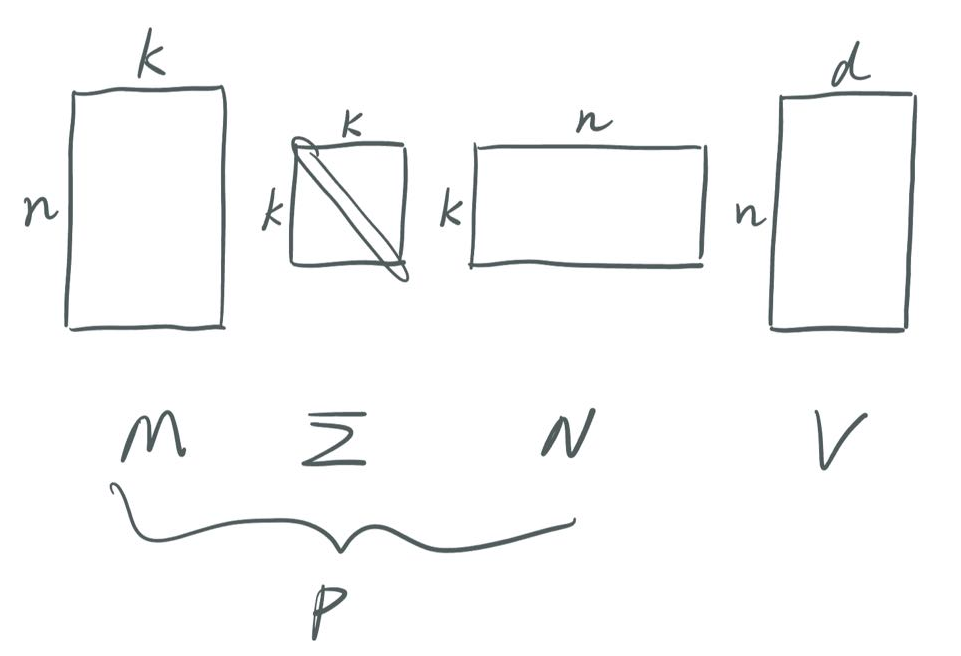
\includegraphics[width=0.5\textwidth]{imgs/5-5.png}
    \caption{Illustration of the Attention Computing using SVD}
    \label{fig:5-5}
\end{figure}

As shown in \ref*{fig:5-5}, we first compute $N V$ in $O(knd)$ time and set result as $X \in \mathbb{R}^{k\times d}$. Because the matrix $\varSigma$ is a diagonal matrix, we can compute $\varSigma X$ in $O(kd)$ time. Suppose the result is $Y \in \mathbb{R}^{k\times d}$. 
Finally, we compute $M Y$ in $O(knd)$ time. The total time complexity is $O(knd + kd + knd) = O(knd)$.
\section{Resnet}
\setcounter{subsection}{1}
\subsection{}
Batch normalization will compute the average and variance of the same channel over the minibatch.
If we use bias in Conv2D, every number of the output in the same channel will be added by a same constant. So, if followed by a batch normalization, the constant will be canceled out when the mean is subtracted. So the bias term won't have any effect.

\newpage

\section{Coding: Image overfitting}
\setcounter{subsection}{4}
\subsection{}

% Resnet code should be submitted on gradescope
% Include plots and results from Q5.5 and written responses for 5.6-8
\subsection{}
The Laplacian is computed by 
\begin{eqnarray}
    \Delta f &=& \frac{\partial^2 f_n}{\partial x \partial y} + \frac{\partial^2 f_n}{\partial y \partial x} \nonumber \\
    f_n &=& \sigma(w_n^T f_{n-1} + b_n) \nonumber \\
    f_{n-1} &=& \sigma(w_{n-1}^T f_{n-2} + b_{n-1}) \nonumber \\
    &\cdots& \nonumber \\
    f_1 &=& \sigma(w_1^T f_0 + b_1) \nonumber \\
    f_0 &=& \sigma(w_0^T \vec{x} + b_0) \nonumber 
\end{eqnarray}

The first order derivative is (for simplicity, we only show the derivative with respect to $x$)
\begin{equation}
    \frac{\partial f}{\partial x} = \frac{\partial f_n}{\partial f_{n-1}} \frac{\partial f_{n-1}}{\partial f_{n-2}} \dots \frac{\partial f_1}{\partial f_0} \frac{\partial f_0}{\partial x} \nonumber
\end{equation}
Because the activation function is ReLu, each term above is whether 0 or $w_i$. So, the first order derivative is just a combination of $w_i$ or 0. To compute the Laplacian, we need to compute derivatives with respect to $y$. We can see the result of the first order derivative is independent of $y$, so the Laplacian is always 0, which results in the all black image.

\subsection{}
We can decrease the learning rate, which is called learning rate decay.

\subsection{}
When training without initialization, the model seems to get stuck in a local minimum. The loss is indeed decreasing, but the output image are just random noise. 

When training without normalization (input coordinates are original integer tuples), the output shows a large scale of variance. I think the reason is that the inputs are too discrete.

\end{document}